\chapter{Verbranding: brandstoffen, reactieproducten en broeikasgassen}\label{ch:g8:combustion-and-fuels}

Een gezin slaapt in een flat waarvan de afvoer van de cv-ketel verstopt
is. De vlam krijgt te weinig \omterm{def:g4:air-a-mixture-of-gases:air}{lucht}, brandt slecht, en een onzichtbaar,
reukloos gas vult langzaam de kamers. Om twee uur 's nachts begint een
kastje aan de muur te gillen: de CO-melder. Iedereen komt op tijd
naar buiten. Dezelfde \omterm{def:g4:what-a-fire-needs:fuel}{brandstof} geeft bij een goede \omterm{def:g4:what-a-fire-needs:burning}{verbranding} alleen
koolstofdioxide en water --- en dat koolstofdioxide heeft zijn eigen
verhaal, geschreven in de \omterm{def:g4:air-a-mixture-of-gases:air}{lucht} van de hele planeet.

\begin{recall}
Een \omterm{def:g4:what-a-fire-needs:burning}{verbranding} heeft een \omterm{def:g4:what-a-fire-needs:fuel}{brandstof}, zuurstof en warmte nodig, en levert
nieuwe stoffen op (\cref{ch:g4:what-a-fire-needs}). \omterm{def:g4:air-a-mixture-of-gases:air}{Lucht} bestaat voor
ongeveer een vijfde uit zuurstof (\cref{ch:g4:air-a-mixture-of-gases}).
Een \omterm{def:g8:balanced-equations:equation}{reactievergelijking} klopt als elke soort \omterm{def:g7:atoms-and-molecules:atom}{atoom} aan beide kanten even
vaak voorkomt (\cref{ch:g8:balanced-equations}).
\end{recall}

\section{Koolstof en methaan verbranden}

\begin{example}[Twee verbrandingen]\label{ex:g8:combustion-and-fuels:two}
Koolstof (houtskool, steenkool) verbrandt tot koolstofdioxide:
\[
  \ce{C(s) + O2(g) -> CO2(g)}.
\]
Methaan, het hoofdbestanddeel van aardgas, verbrandt tot koolstofdioxide
en water:
\[
  \ce{CH4(g) + 2O2(g) -> CO2(g) + 2H2O(l)}.
\]
In beide gevallen wordt kalkwater troebel met het gevormde gas; bij
methaan beslaat bovendien een koud glas.
\end{example}

\begin{method}[De verbranding opschrijven van een brandstof uit koolstof en waterstof]\label{met:g8:combustion-and-fuels:write}
Voor een \omterm{def:g4:what-a-fire-needs:fuel}{brandstof} waarvan de \omterm{def:g7:atoms-and-molecules:molecule}{moleculen} alleen koolstof en waterstof
bevatten:
\begin{enumerate}
  \item de \omterm{def:g7:chemical-reactions:reactant}{reactieproducten} zijn koolstofdioxide en water;
  \item maak koolstof kloppend met \ce{CO2}, daarna waterstof met
        \ce{H2O};
  \item tel de zuurstofatomen rechts en maak ze kloppend met \ce{O2};
        verdubbel alles als er een half verschijnt.
\end{enumerate}
Voor butaan: \ce{2C4H10 + 13O2 -> 8CO2 + 10H2O}.
\end{method}

\section{Volledige en onvolledige verbranding}

\begin{definition}[Volledige en onvolledige verbranding]\label{def:g8:combustion-and-fuels:complete}
Een \emph{volledige verbranding}\index{volledige verbranding} vindt
plaats met genoeg zuurstof: alle koolstof van de \omterm{def:g4:what-a-fire-needs:fuel}{brandstof} wordt
koolstofdioxide. Een \emph{onvolledige verbranding}\index{onvolledige verbranding}
vindt plaats met te weinig zuurstof: een deel van de koolstof wordt
koolstofmono-oxide, \ce{CO}, of roet, dat koolstof is, \ce{C}.
\end{definition}

\begin{example}[Methaan met te weinig zuurstof]\label{ex:g8:combustion-and-fuels:incomplete}
Met te weinig \omterm{def:g4:air-a-mixture-of-gases:air}{lucht} kan methaan \omterm{def:g4:what-a-fire-needs:burning}{verbranden} tot koolstofmono-oxide of tot
roet:
\[
  \ce{2CH4 + 3O2 -> 2CO + 4H2O}, \qquad \ce{CH4 + O2 -> C + 2H2O}.
\]
\end{example}

\begin{proposition}[Een vlam aflezen]\label{prop:g8:combustion-and-fuels:flame}
Een bunsenbrander met open luchtgat \omterm{def:g2:mixing-and-dissolving:mix}{mengt} \omterm{def:g4:air-a-mixture-of-gases:air}{lucht} door het gas voordat het
verbrandt: de vlam is blauw en nauwelijks zichtbaar, de \omterm{def:g4:what-a-fire-needs:burning}{verbranding}
volledig. Met het luchtgat dicht vindt het gas te weinig zuurstof: de
vlam is geel en walmt, en een koud voorwerp dat je erin houdt, wordt
zwart van het roet --- de \omterm{def:g4:what-a-fire-needs:burning}{verbranding} is onvolledig.
\end{proposition}

\begin{omfigure}
\begin{tikzpicture}[font=\small, scale=1.3]
  \pic[transform shape] at (0,0) {bunsen=open};
  \node[anchor=north, align=center] at (0,-0.1) {luchtgat open:\\ blauwe vlam, volledig};
  \pic[transform shape] at (4,0) {bunsen=closed};
  \node[anchor=north, align=center] at (4,-0.1) {luchtgat dicht:\\ gele vlam, onvolledig};
  \draw[<-, omProp, thick] (0.08,0.6) -- (1.4,0.9) node[right, text=black] {luchtgat};
  \draw[<-, omProp, thick] (-0.4,0.3) -- (-1.3,0.6) node[left, text=black] {gas};
  \draw[<-, omProp, thick] (4.15,3.3) -- (5.0,3.5) node[right, text=black, align=left]
    {roet, koolstof-\\ mono-oxide};
\end{tikzpicture}

{\small Een bunsenbrander. \omterm{def:g4:air-a-mixture-of-gases:air}{Lucht} die onderaan binnenkomt, geeft een blauwe
vlam en een \omterm{def:g8:combustion-and-fuels:complete}{volledige verbranding}; zonder die \omterm{def:g4:air-a-mixture-of-gases:air}{lucht} is de vlam geel en
walmend.}
\end{omfigure}

\begin{omfigure}
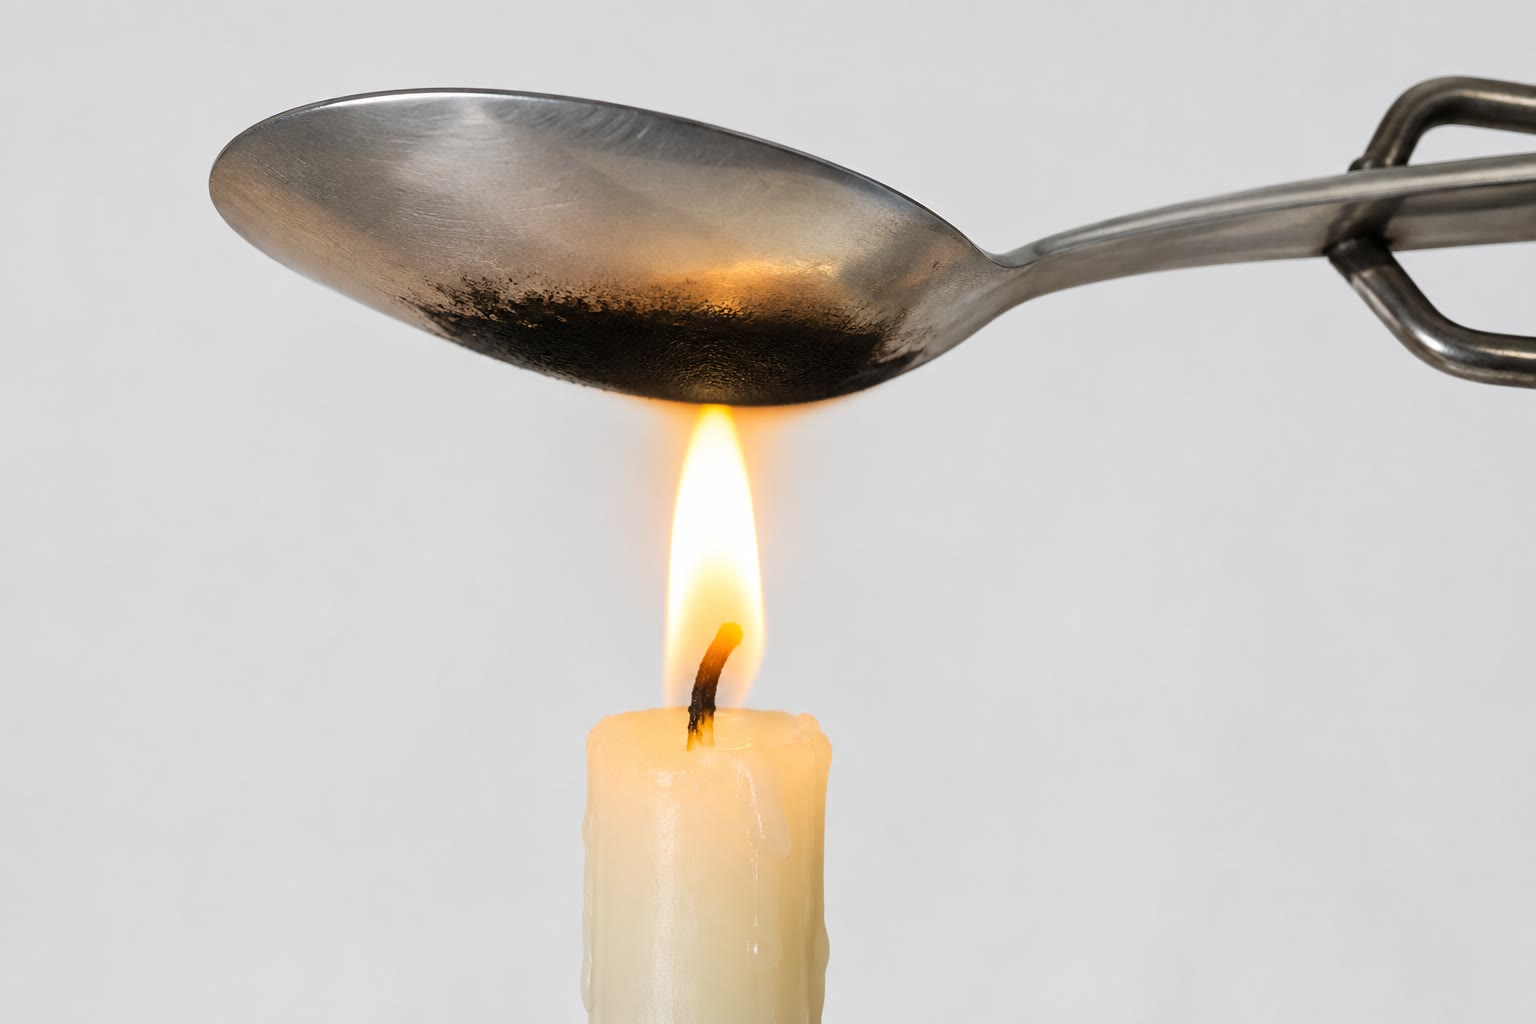
\includegraphics[width=0.45\linewidth]{images/book1/ai/g8-soot-spoon.jpg}

{\small Een koude lepel in een gele kaarsvlam wordt zwart van het roet:
de \omterm{def:g4:what-a-fire-needs:burning}{verbranding} is onvolledig.}
\end{omfigure}

\section{Koolstofmono-oxide, een stil gevaar}

\begin{proposition}[Waarom koolstofmono-oxide dodelijk is]\label{prop:g8:combustion-and-fuels:co}
Koolstofmono-oxide heeft geen kleur, geen geur en geen smaak. Als je het
inademt, neemt het de plaats in van zuurstof in het bloed (het
biologieboek legt uit hoe), met hoofdpijn en slaperigheid tot gevolg, en
in een afgesloten ruimte bewusteloosheid en de dood. Het ontstaat bij
elke \omterm{def:g4:what-a-fire-needs:fuel}{brandstof} die met te weinig \omterm{def:g4:air-a-mixture-of-gases:air}{lucht} verbrandt: een cv-ketel of geiser
die slecht onderhouden is of een verstopte afvoer heeft, een brander in
een gesloten tent, een barbecue of een aggregaat dat binnen gebruikt
wordt.
\end{proposition}

\begin{safety}{\ghs[0.8cm]{GHS02}\ghs[0.8cm]{GHS04}\ghs[0.8cm]{GHS06}\ghs[0.8cm]{GHS08}}
% ledger: ghs:CO
Koolstofmono-oxide: zeer licht ontvlambaar gas (GHS02), geleverd onder
druk (GHS04); giftig bij inademing (GHS06); veroorzaakt schade aan
organen bij herhaalde blootstelling en kan het ongeboren kind schaden
(GHS08).
\end{safety}

\begin{remark}[Vergiftiging voorkomen]\label{rem:g8:combustion-and-fuels:prevent}
Gastoestellen worden regelmatig door een vakman onderhouden, afvoeren en
ventilatieroosters worden nooit afgedekt, barbecues en aggregaten worden
alleen buiten gebruikt, en bij elke brander hangt een CO-melder.
\end{remark}

\begin{omfigure}
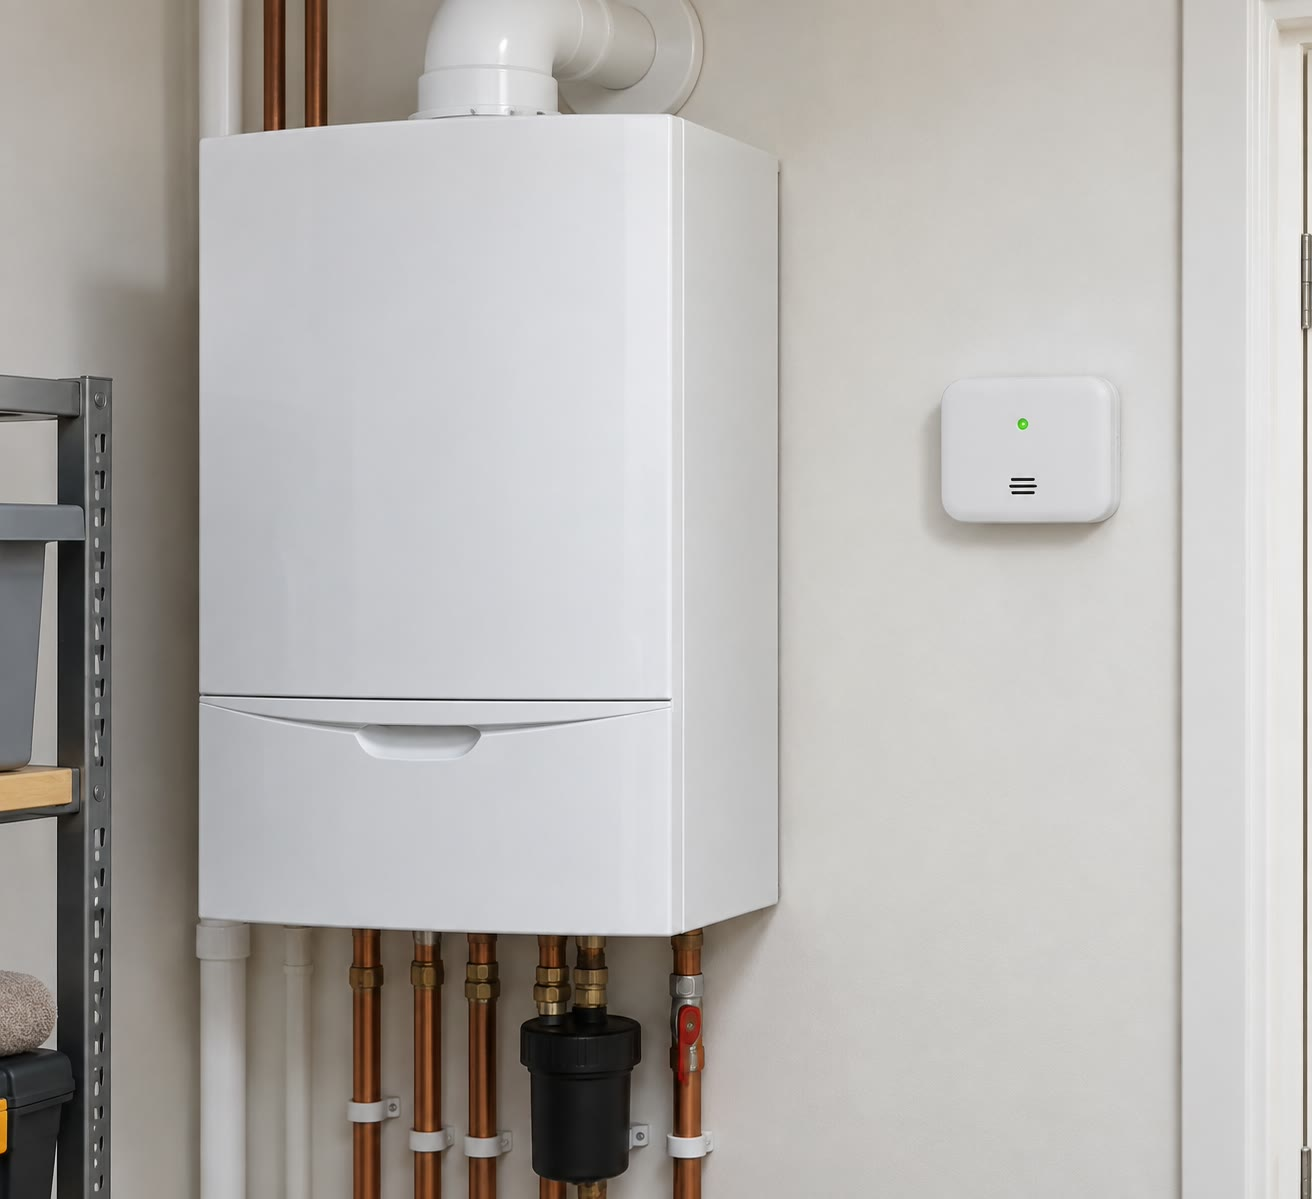
\includegraphics[width=0.45\linewidth]{images/book1/ai/g8-boiler-alarm.jpg}

{\small Een cv-ketel en, ernaast, een CO-melder.}
\end{omfigure}

\section{Koolstofdioxide en het broeikaseffect}

\begin{definition}[Broeikasgas]\label{def:g8:combustion-and-fuels:greenhouse}
Een \emph{broeikasgas}\index{broeikasgas} is een gas in de \omterm{def:g4:air-a-mixture-of-gases:air}{lucht} dat het
zonlicht doorlaat maar een deel van de warmte tegenhoudt die het
aardoppervlak terugstuurt naar de ruimte, en zo de onderste lagen van de
atmosfeer verwarmt. Waterdamp, koolstofdioxide en methaan zijn
broeikasgassen; stikstof en zuurstof niet. (Hoe dat werkt, staat in het
natuurkundeboek.)
\end{definition}

\begin{proposition}[Er komt steeds meer koolstofdioxide in de lucht]\label{prop:g8:combustion-and-fuels:rising}
% ledger: co2:mlo-1959, co2:mlo-2025 (rise 111.4 ppm, +35 %)
De hoeveelheid koolstofdioxide in de \omterm{def:g4:air-a-mixture-of-gases:air}{lucht} wordt sinds 1959 zonder
onderbreking gemeten in een observatorium op een berg midden in de
Grote Oceaan. Ze bedroeg 316 deeltjes per miljoen (ppm) \omterm{def:g4:air-a-mixture-of-gases:air}{lucht} in 1959 en
427 ppm in 2025: een stijging van ongeveer \qty{35}{\percent} in één
mensenleven, vooral door het \omterm{def:g4:what-a-fire-needs:burning}{verbranden} van steenkool, aardolie en
aardgas. Het extra koolstofdioxide versterkt het broeikaseffect en
verwarmt het klimaat.
\end{proposition}

\begin{omfigure}
\begin{tikzpicture}
\begin{axis}[width=0.85\linewidth, height=6cm, xmin=1955, xmax=2030,
    ymin=300, ymax=440, xlabel={jaar}, ylabel={koolstofdioxide (ppm)},
    axis lines*=left, ymajorgrids, grid style={gray!20},
    tick label style={font=\small, /pgf/number format/1000 sep={}},
    label style={font=\small}]
\addplot[omDef, thick, mark=*, mark size=0.8pt]
  table[x=year, y=ppm] {figdata/out/grade-8-co2-record.dat};
\node[anchor=west, font=\small] at (axis cs:1962,306) {316 ppm in 1959};
\node[anchor=east, font=\small] at (axis cs:2023,428) {427 ppm in 2025};
\end{axis}
\end{tikzpicture}

{\small Jaargemiddelde van het koolstofdioxide in de \omterm{def:g4:air-a-mixture-of-gases:air}{lucht}, gemeten sinds
1959 (gegevens van het NOAA Global Monitoring Laboratory; vóór 1974 van
het Scripps Institution of Oceanography).}
\end{omfigure}

\section{Fossiele en hernieuwbare brandstoffen}

\begin{definition}[Fossiele en hernieuwbare brandstoffen]\label{def:g8:combustion-and-fuels:fossil}
Een \emph{fossiele brandstof}\index{fossiele brandstof} --- steenkool,
aardolie, aardgas --- is in de loop van miljoenen jaren onder de grond
ontstaan uit de resten van oeroude planten en zeedieren. Een
\emph{hernieuwbare brandstof}\index{hernieuwbare brandstof} wordt
gemaakt van planten die nu groeien, of van afval: hout, biogas uit mest
en etensresten, ethanol uit suikerbieten of suikerriet.
\end{definition}

\begin{proposition}[Waar de koolstof vandaan komt]\label{prop:g8:combustion-and-fuels:cycle}
Planten halen koolstofdioxide uit de \omterm{def:g4:air-a-mixture-of-gases:air}{lucht} om te groeien. Als je een
\omterm{def:g8:combustion-and-fuels:fossil}{hernieuwbare brandstof} verbrandt, geef je koolstofdioxide terug dat de
planten een paar jaar eerder uit de \omterm{def:g4:air-a-mixture-of-gases:air}{lucht} hebben gehaald. Als je een
\omterm{def:g8:combustion-and-fuels:fossil}{fossiele brandstof} verbrandt, komt koolstof vrij die miljoenen jaren
onder de grond opgesloten zat: dat voegt koolstofdioxide toe aan de
\omterm{def:g4:air-a-mixture-of-gases:air}{lucht}.
\end{proposition}

\begin{omfigure}
\begin{tikzpicture}[font=\small,
    box/.style={draw=omDef, fill=omDef!6, rounded corners=2pt, align=center,
      minimum height=0.9cm, text width=2.6cm}]
  \node[box] (air) at (0,3) {koolstofdioxide\\ in de lucht};
  \node[box] (plants) at (5.6,3) {planten groeien\\ (nemen \ce{CO2} op)};
  \node[box] (fuel) at (5.6,0.4) {hout, biogas,\\ bio-ethanol};
  \node[box, draw=black!50, fill=black!8] (fossil) at (0,0.4) {steenkool, olie, gas:\\ onder de grond};
  \draw[->, thick, omProp] (air) -- (plants);
  \draw[->, thick, omProp] (plants) -- (fuel);
  \draw[->, thick, omProp] (fuel) -- (air);
  \node[text=black, font=\footnotesize, align=left, anchor=north west] at (1.5,1.45)
    {verbranding,\\ na een paar jaar};
  \draw[->, thick, black!60] (fossil) -- node[midway, left, text=black, font=\footnotesize,
    align=right] {verbranding:\\ miljoenen jaren\\ oude koolstof} (air);
\end{tikzpicture}

{\small \omterm{def:g8:combustion-and-fuels:fossil}{Hernieuwbare brandstoffen} geven de \omterm{def:g4:air-a-mixture-of-gases:air}{lucht} de koolstof terug die
hun planten eruit haalden; \omterm{def:g8:combustion-and-fuels:fossil}{fossiele brandstoffen} voegen koolstof toe die
onder de grond opgeslagen was.}
\end{omfigure}

\begin{omfigure}
\begin{minipage}[t]{0.48\linewidth}\centering
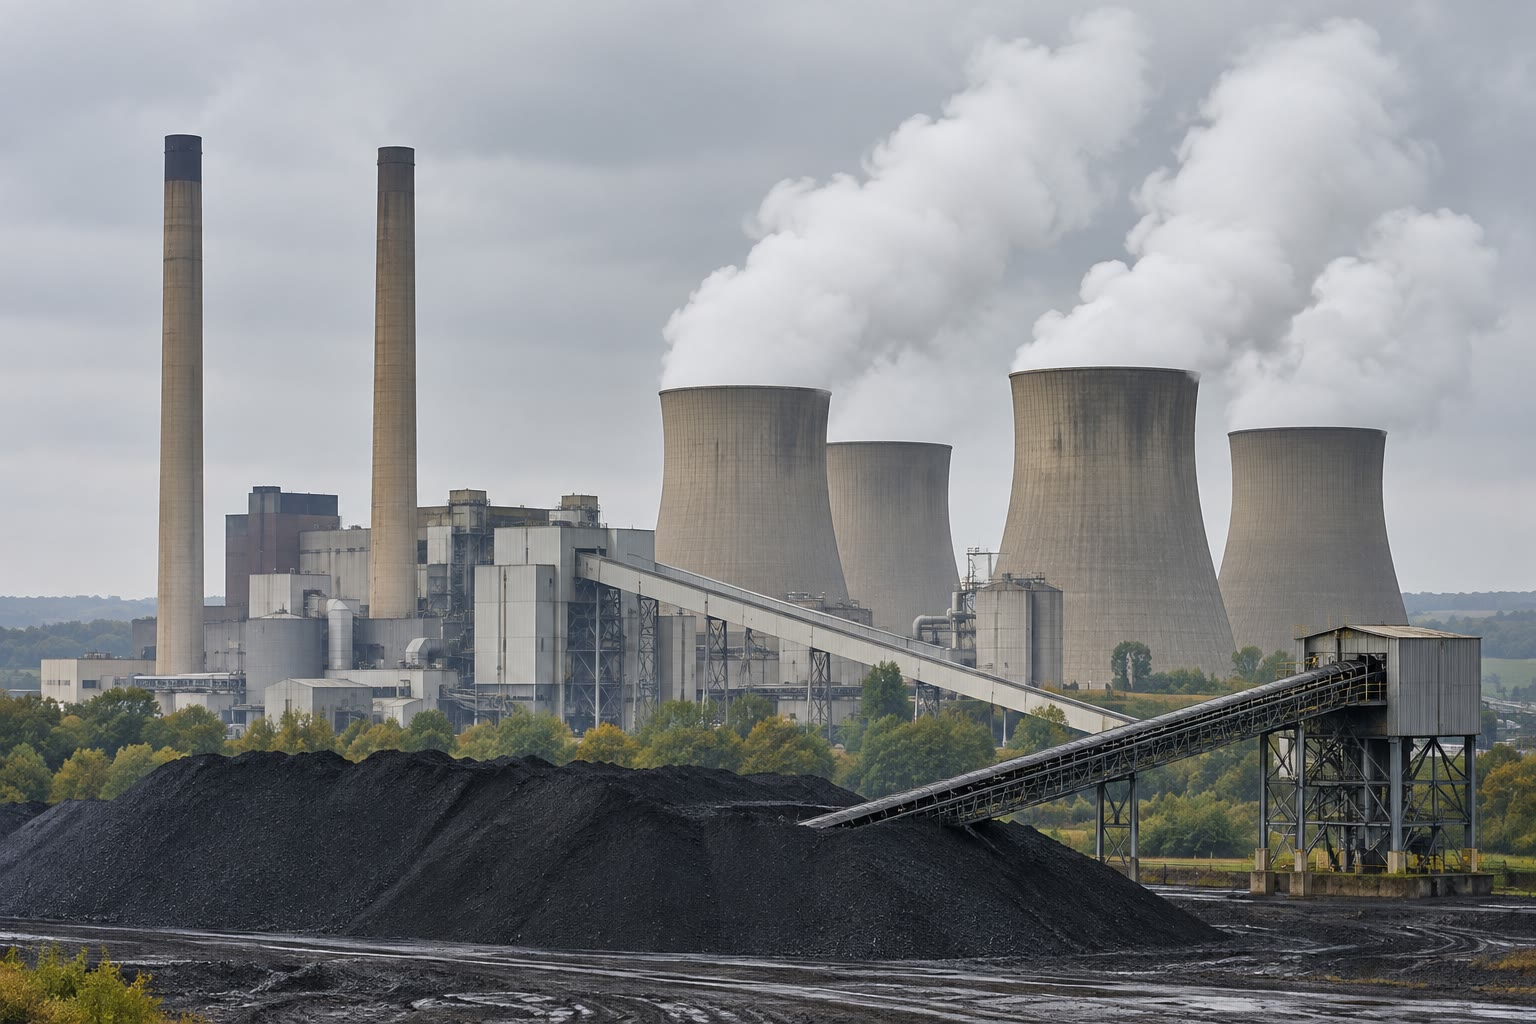
\includegraphics[width=\linewidth,height=4.6cm,keepaspectratio]{images/book1/ai/g8-coal-plant.jpg}

{\small Een kolencentrale.}
\end{minipage}\hfill
\begin{minipage}[t]{0.48\linewidth}\centering
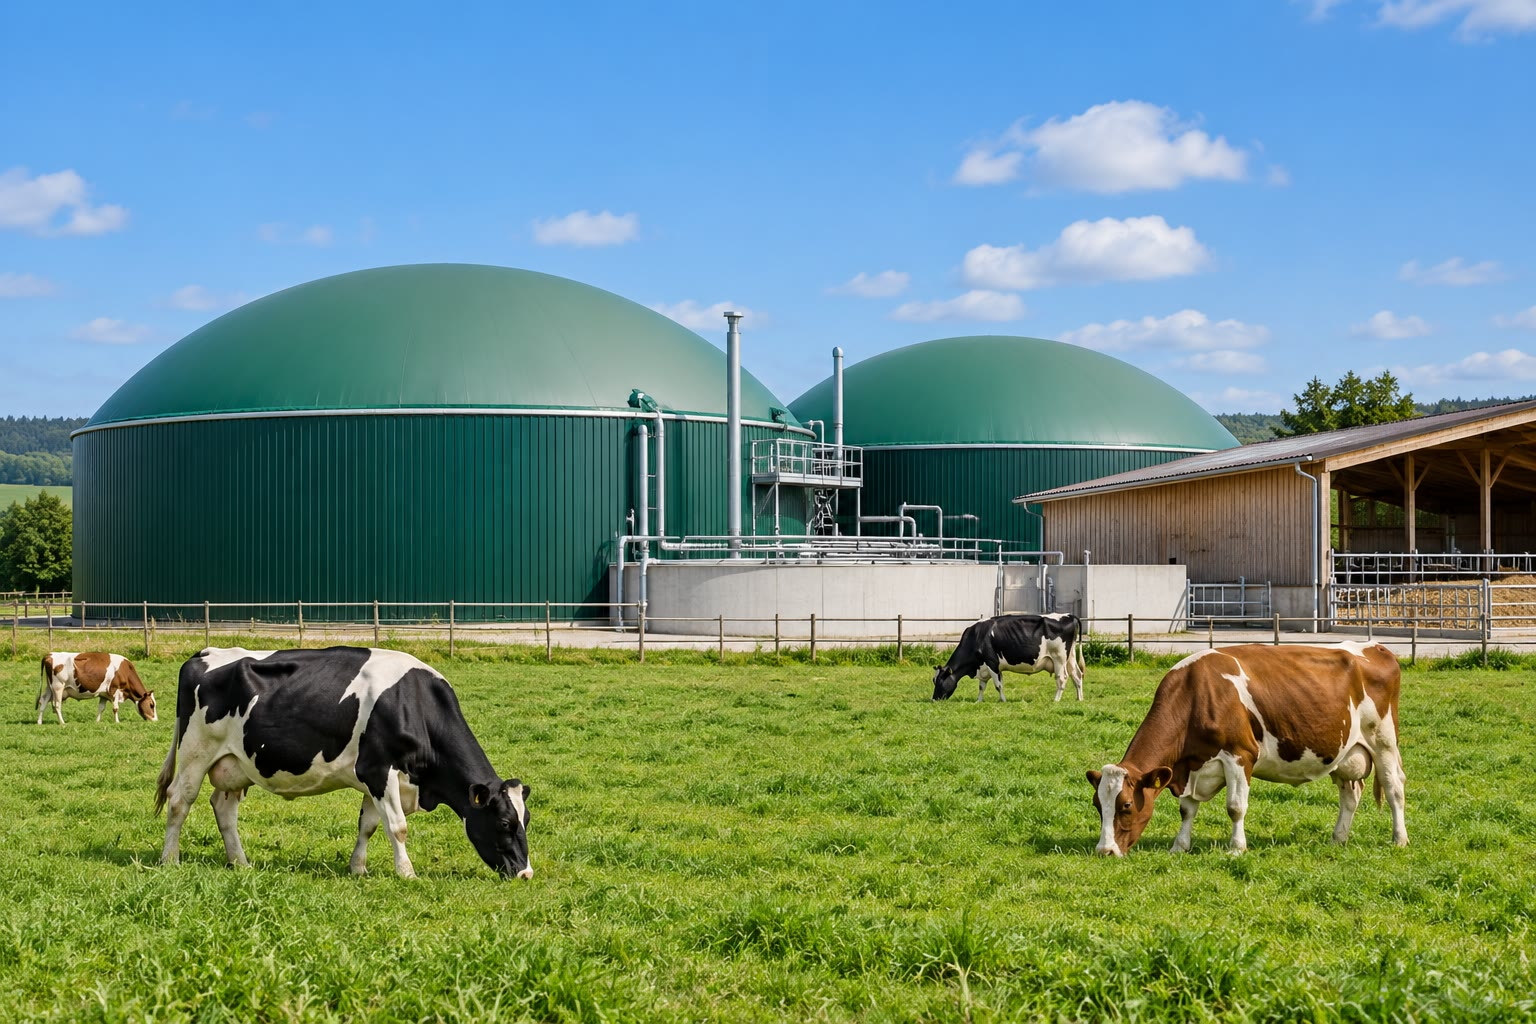
\includegraphics[width=\linewidth,height=4.6cm,keepaspectratio]{images/book1/ai/g8-biogas-farm.jpg}

{\small Een biogasinstallatie op een boerderij: mest wordt een
\omterm{def:g8:combustion-and-fuels:fossil}{hernieuwbare brandstof}.}
\end{minipage}
\end{omfigure}

\section{Oefeningen}

\begin{exercise}[$\star$]\label{exo:g8:combustion-and-fuels:1}
Schrijf de \omterm{def:g8:balanced-equations:equation}{kloppende reactievergelijking} op van de \omterm{def:g8:combustion-and-fuels:complete}{volledige verbranding}
van koolstof.
\end{exercise}

\begin{exercise}[$\star$]\label{exo:g8:combustion-and-fuels:2}
Wat is het verschil tussen een volledige en een \omterm{def:g8:combustion-and-fuels:complete}{onvolledige verbranding}?
\end{exercise}

\begin{exercise}[$\star$]\label{exo:g8:combustion-and-fuels:3}
Waarom wordt koolstofmono-oxide een stil gevaar genoemd?
\end{exercise}

\begin{exercise}[$\star$]\label{exo:g8:combustion-and-fuels:4}
Fossiel of hernieuwbaar: steenkool, hout, aardgas, biogas, benzine,
ethanol uit suikerbieten?
\end{exercise}

\begin{exercise}[$\star\star$]\label{exo:g8:combustion-and-fuels:5}
Schrijf de \omterm{def:g8:balanced-equations:equation}{kloppende reactievergelijking} op van de \omterm{def:g8:combustion-and-fuels:complete}{volledige verbranding}
van propaan, \ce{C3H8}.
\end{exercise}

\begin{exercise}[$\star\star$]\label{exo:g8:combustion-and-fuels:6}
Ethanol, \ce{C2H6O}, verbrandt volledig in zuurstof. Maak
\ce{C2H6O + O2 -> CO2 + H2O} kloppend. % ce-unbalanced-ok (to balance)
\end{exercise}

\begin{exercise}[$\star\star$]\label{exo:g8:combustion-and-fuels:7}
Een pan boven een gele vlam wordt aan de onderkant zwart. Wat is de
zwarte stof? Wat zegt dat over de \omterm{def:g4:what-a-fire-needs:burning}{verbranding}?
\end{exercise}

\begin{exercise}[$\star\star$]\label{exo:g8:combustion-and-fuels:8}
Lees de koolstofdioxidecurve af: hoeveel koolstofdioxide bevatte de \omterm{def:g4:air-a-mixture-of-gases:air}{lucht}
ongeveer in 1980 en in 2000? Met hoeveel ppm steeg het in die twintig
jaar?
\end{exercise}

\begin{exercise}[$\star\star$]\label{exo:g8:combustion-and-fuels:9}
Waarom voegt het \omterm{def:g4:what-a-fire-needs:burning}{verbranden} van hout op den duur minder koolstofdioxide
toe aan de \omterm{def:g4:air-a-mixture-of-gases:air}{lucht} dan het \omterm{def:g4:what-a-fire-needs:burning}{verbranden} van steenkool, hoewel beide
koolstofdioxide opleveren?
\end{exercise}

\begin{exercise}[$\star\star$]\label{exo:g8:combustion-and-fuels:10}
Maak de \omterm{def:g8:combustion-and-fuels:complete}{onvolledige verbranding} van koolstof tot koolstofmono-oxide
kloppend, \ce{C + O2 -> CO}. % ce-unbalanced-ok (to balance)
\end{exercise}

\begin{exercise}[$\star\star\star$]\label{exo:g8:combustion-and-fuels:11}
Met welk percentage is het koolstofdioxide in de \omterm{def:g4:air-a-mixture-of-gases:air}{lucht} gestegen van 1959
(316 ppm) tot 2025 (427 ppm)? Rond af op een geheel getal.
\end{exercise}

\begin{exercise}[$\star\star\star$]\label{exo:g8:combustion-and-fuels:12}
Een gaskachel brandt in een kleine kamer met het raam dicht. Leg met
twee \omterm{def:g8:balanced-equations:equation}{reactievergelijkingen} uit dit hoofdstuk uit hoe de \omterm{def:g4:what-a-fire-needs:burning}{verbranding} na
verloop van tijd van volledig onvolledig kan worden, en waarom dat
gevaarlijk is.
\end{exercise}

\section{Probleem: De brander in de tent}

\begin{problem}[{Weekendprobleem --- een kampeerbrander, het gas dat hij
verbrandt, wat hij oplevert, en waarom hij nooit in een tent hoort}]
\label{pb:g8:combustion-and-fuels:1}
% ledger: ghs:propane
Een kampeerbrander verbrandt propaan, \ce{C3H8}, uit een busje dat er
\qty{450}{g} van bevat. In de open \omterm{def:g4:air-a-mixture-of-gases:air}{lucht} is de vlam blauw. Gebruik deze
massaverhouding, berekend uit de \omterm{def:g8:balanced-equations:equation}{kloppende reactievergelijking}:
\qty{44}{g} propaan die volledig verbrandt, geeft \qty{132}{g}
koolstofdioxide.

\medskip
\noindent\textbf{Deel I --- De \omterm{def:g8:balanced-equations:equation}{reactievergelijkingen}.}
\begin{enumerate}
  \item Schrijf de \omterm{def:g8:balanced-equations:equation}{kloppende reactievergelijking} op van de \omterm{def:g8:combustion-and-fuels:complete}{volledige
        verbranding} van propaan.
  \item Controleer haar door aan elke kant de \omterm{def:g7:atoms-and-molecules:atom}{atomen} van elke soort te
        tellen.
  \item Maak de \omterm{def:g8:combustion-and-fuels:complete}{onvolledige verbranding}
        \ce{C3H8 + O2 -> CO + H2O} kloppend. % ce-unbalanced-ok (to balance)
  \item Welke van de twee heeft per propaanmolecuul meer zuurstof nodig?
\end{enumerate}

\medskip
\noindent\textbf{Deel II --- In een tent.}
\begin{enumerate}[resume]
  \item Een brander die in een gesloten tent wordt aangestoken, brandt al
        snel met een gele vlam. Leg uit waarom.
  \item Welk gevaarlijk gas ontstaat er dan? Geef twee eigenschappen
        waardoor je het moeilijk opmerkt.
  \item Op het propaanbusje staan twee pictogrammen. Noem ze en zeg wat
        elk betekent.
  \item Geef twee regels om een kampeerbrander veilig te gebruiken.
\end{enumerate}

\medskip
\noindent\textbf{Deel III --- Het koolstofdioxide van één busje.}
\begin{enumerate}[resume]
  \item Hoeveel keer zwaarder is het gevormde koolstofdioxide dan het
        verbrande propaan?
  \item Waar komen de extra grammen vandaan?
  \item Is propaan een fossiele of een \omterm{def:g8:combustion-and-fuels:fossil}{hernieuwbare brandstof}? Voegt het
        \omterm{def:g4:what-a-fire-needs:burning}{verbranden} ervan koolstofdioxide toe aan de \omterm{def:g4:air-a-mixture-of-gases:air}{lucht}?
  \item Bereken de massa koolstofdioxide die vrijkomt als een heel busje
        van \qty{450}{g} volledig verbrandt.
\end{enumerate}
\end{problem}
